\chapter{Image processing using the graph Laplacian operator}

\paragraph{}
Multiple image processing filters can be built using the graph Laplacian operator.
As Milanfar mentions in \cite{siam_slides_2016}, smoothing, deblurring, sharpening, dehazing, and other filters can be created.
Laplacian operators can also be used as the basis for compression artifact removal, low-light imaging and image segmentation.

We shall consider an adapted version of the proposed algorithm in \cite{glide_2014} to solve the eigenvalue problem by solving linear systems.
Let's first introduce step-by-step the algorithm, then the possible variations and finally our parallel implementation.

\section{Algorithm}

\paragraph{}
An image filter consists of a function which outputs one pixel, taking all pixels as input and applying weights to them. We can write this as
\[z_i = \sum_j W_{ij}y_j,\]
\(z_i\) being the output pixel, \(W_{ij}\) the weight and \(y_j\) all input pixels.
This means that a vector of weights exists for each pixel.

As a practical notation, we can say that, with \(W\) the matrix of weights and \(y\) the input image as a vector,
\[z = Wy.\]
The filter matrix \(W\) considered here is data-dependent and built upon the input image \(y\).

\paragraph{Image as graph}
Let's think of an image as a graph.
Each pixel is a node and has edges to other nodes.
The simplest way to connect pixels to other pixels is their direct neighbours, in which case each node has four edges.
To avoid losing any information, we will instead consider the case of a complete graph, each node connects to all other nodes.

To preserve the image information in the graph, the graph edges will be assigned a weight, measuring the similarity\footnote{Also called affinity.} between the two nodes, thus between two pixels.
There are multiple ways the similarity can be defined.

The most intuitive definition considers spatial proximity.
This means that similar pixels are spatially close, which, translated to a basic filter, is the same as a Gaussian filter which computes a weighted average of the pixel's neighbourhood and produces what is known as Gaussian blur.
Another similarity definition is to consider the pixel's color.
A good compromise is to consider an average of both, spatial and color closeness, with a certain weighting.

From this definition can be computed the adjacency matrix of the graph taking into account the edge weights.
We will call this matrix the affinity matrix\footnote{Or similarity matrix, or kernel matrix}\ \(K\) which represents the similarity of each pixel to every other pixel in the image.
Consequently, this matrix is symmetric and of size \(N \times N\) with \(N\) the number of pixels in the image, and, depending on the similarity function, bounds on the values of \(K\).

Using this affinity matrix, we obtain the graph Laplacian \(\Lapl\), used to build the filter matrix \(W\).

\paragraph{Building the filter}

Multiple graph Laplacian definitions, more or less equivalent, exist and can have slightly different properties.
In the case of image smoothing, the filter \(W\) is defined such as \(\Lapl = I - W\) \cite{siam_slides_2016} and so \(W = I - \Lapl\).

However, all these matrices \(K\), \(\Lapl\) and \(W\) represent huge computational costs.
Only storing one of these matrices is already a challenge since they have a size of \(N^2\).

For example, a tiny test image of size \(256 \times 256\) has 65 536 pixels, so one of these matrices has approximately \(4.29 \times 10^9\) elements.
Considering storing those with a 64 bits type, one matrix takes more than 34 GB of memory.
Scaling to an everyday-smartphone picture, taken with a 10 MPixel camera, a matrix contains \(10^{14}\) elements, meaning 800 TB of memory.

\paragraph{Approximation by sampling and Nystr\"om extension}

To avoid storing any of those huge matrices, approximation will be necessary.
It starts by sampling the image and only select a subset of \(p\) pixels, with \(p \ll N\).
Numerically, \(p\) should represent around 1\% or less of the image pixels \cite{fowlkes_spectral_2004}.
The rows and columns of the matrix \(K\) are re-organised such as
\[K = \begin{bmatrix}K_A & K_B \\ K_B^T & K_C\end{bmatrix}\]
with \(K_A\) being the affinities between the sampled pixels and thus of size \(p \times p\).
\(K_B\) holds the affinities between the sampled pixels and the remaining pixels and is therefore of size \(p \times (N-p)\).
Finally, the submatrix \(K_C\) contains the similarities between the remaining pixels.
Knowing that \(K_C\) is of size \((N-p) \times (N-p)\) and that \(p \ll N\), this submatrix is huge.

To have a numerical approximation of a symmetric matrix \(K\), we use the eigendecomposition:
\[K = \Phi \Pi \Phi^T\]
where \(\Phi\) are the orthonormal eigenvectors of \(K\) stored as a matrix and \(\Pi\) contains the eigenvalues of \(K\).
\cite{fowlkes_spectral_2004} suggests the Nystr\"om extension to approximate \(K\) by \(\tilde{K} = \tilde{\Phi} \tilde{\Pi} \tilde{\Phi^T}\), with \(\tilde{\Pi} = \Pi_A\) and the first \(m\) eigenvectors:
\[\tilde{\Phi} = \begin{bmatrix}\Phi_A \\ K_B^T \Phi_A \Pi_A^{-1}\end{bmatrix}\]
with the eigendecomposition \(K_A = \Phi_A \Pi_A \Phi_A^T\).
We note that the number of computed eigenvalues of \(K_A\) is \(m\) with \(m \le p\).
It is not required to compute all eigenvalues of the sampled pixels matrix because \(p\) can still be large if the input image has a high resolution.
The approximated matrix would be of the form \cite{glide_2014}
\[\tilde{K} = \begin{bmatrix}K_A & K_B \\ K_B^T & K_B^T K_A^{-1} K_B\end{bmatrix}.\]
We can clearly see that the huge submatrix \(K_C\) is now approximated.

\paragraph{Eigendecomposition}
We need to compute the largest eigenvalues of the filter \(W\).
For the approximation, we will actually need to compute the largest eigenvalues of the sampled pixels of the filter \(W_A\) to use the Nystr\"om extension.
Considering a small sample to compute the largest eigenvalues works to approximate the complete filter because these eigenvalues are decaying rapidly as shows the figure below:
\begin{figure}[H]
  \centering
  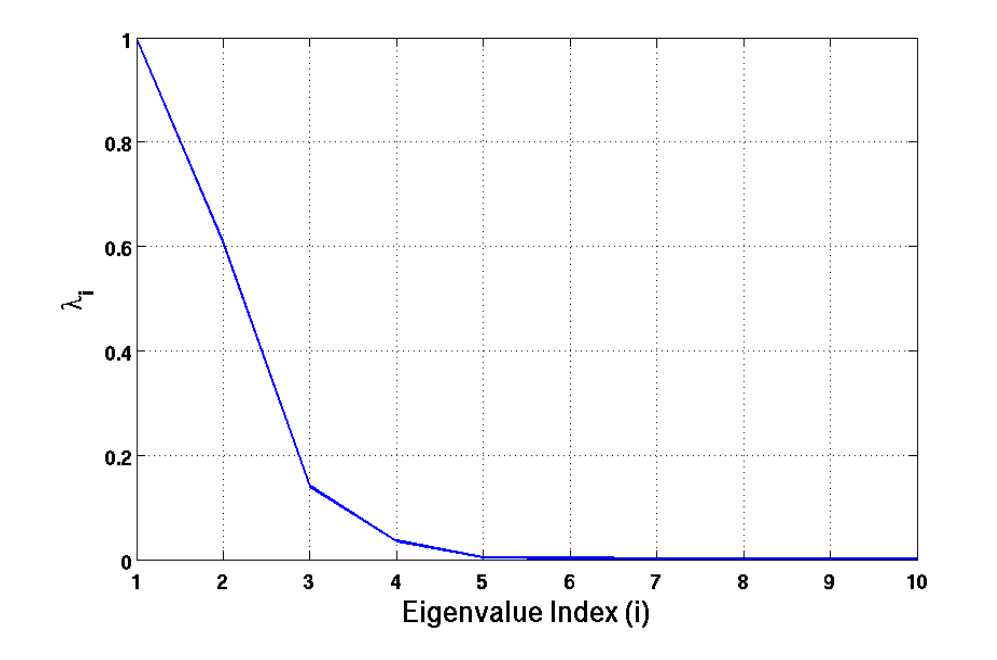
\includegraphics[width=0.9\textwidth]{img/decayingEigenvalues.png}
  \caption{Largest eigenvalues of an image filter, taken from \cite{siam_slides_2016}.}
\end{figure}

We know that the eigenvalues of submatrix\ \(W_A\) are between the extremum eigenvalues of the filter, which is known as the interlacing property of principal submatrices.
We also know that computing the largest eigenvalues of the submatrix filter is equivalent to computing the smallest eigenvalues of the corresponding submatrix of the Laplacian operator.
The proofs to these statements can be found in Appendix \ref{appendix:eigenvalue_proof}.

The goal of this observation is the way of computing the eigenvalues.
For the largest eigenvalues, the most famous algorithm is the power method.
For the smallest eigenvalues, the inverse power method is usually used.
The latter requires either to invert a matrix, or to solve a linear system.
We will solve systems of linear equations to compute the first eigenvalues of the Laplacian in order to observe the behavior of solvers on these dense matrices.

So our approximated Laplacian eigendecomposition, using the Nystr\"om extension and eigendecomposition of \(\Lapl_A\):
\[\tilde{\Lapl} = \tilde{\Phi} \tilde{\Pi} \tilde{\Phi^T}.\]

\paragraph{Output image}
\cite{modern_tour_2013} defines the filter as \(W = I - \Lapl\) and therefore the output image using the filter approximation \(\tilde{W}\) can be expressed as:
\begin{equation}
 \begin{split}
     \tilde{z} & = \tilde{W}y \\
               & = (I - \tilde{\Lapl}) y \\
               & = (I - \tilde{\Phi} \tilde{\Pi} \tilde{\Phi^T}) y \\
               & = y - \tilde{\Phi} \tilde{\Pi} \tilde{\Phi^T} y
 \end{split}
\end{equation}

\begin{algorithm}[H]
 \caption{Image processing using graph Laplacian operator}
 \begin{algorithmic}
  \REQUIRE \(y\) an image of size \(n \times m\)
  \ENSURE \(z\) the output image
  \STATE \(N \leftarrow n*m\)
  \STATE \COMMENT{Sampling}
  \STATE Sample \(p\) pixels, \(p \ll N\)
  \STATE \COMMENT{Kernel matrix approximation}
  \STATE Compute \(K_A\) (size \(p \times p\)) and \(K_B\) (size \(p \times (N-p)\)) such as \(K = \begin{bmatrix} K_A & K_B \\ K_B^T & K_C \end{bmatrix}\)
  \STATE Compute the Laplacian \(\Lapl_A\) and \(\Lapl_B\)
  \STATE \COMMENT{Eigendecomposition}
  \STATE Compute the smallest eigenvalues \(\Pi_A\) and the associated eigenvectors \(\Phi_A\) of \(\Lapl_A\)
  \STATE Nystr\"om extension \(\tilde{\Phi} \leftarrow \begin{bmatrix} \Phi_A \\ \Lapl_B^T \Phi_A \Pi_A^{-1} \end{bmatrix}\)
  \STATE \COMMENT{Apply the filter}
  \STATE \(\tilde{z} \leftarrow y - \tilde{\Phi} \Pi_A \tilde{\Phi^T} y\)
 \end{algorithmic}
\end{algorithm}

\section{Variations}

\paragraph{}
Multiple steps in this algorithm are to be defined in contrete terms to implement it.
For each, several methods exists, with different properties.
We present some of these methods for each step.

\subsection{Sampling method}

\paragraph{}
The sample requires to represent only less than 1\% of the pixels of the image \cite{fowlkes_spectral_2004}.
To achieve this, we can use different approaches.
The chosen method is decisive for the application of the Nystr\"om method.
\begin{description}[align=left]
 \item [Random sampling (RS)] most common and simple sampling scheme, but no deterministic guarantee of the output quality. It can produce good results for images with poor resolution, but with a huge amount of data, random sampling is limited because it cannot reflect the structure of the data set \cite{zhan_improved_2017}.
 \item [K-means sampling (KS)] associate to each pixel a 5-D space (R, G, B, X, Y) and divide the pixels into K clusters (K centers). These clusters are a good sampling scheme for images with simple and uniform backgrounds \cite{kao_sampling_2012} \cite{zhang_improved_2008}.
 \item [Uniform spatially sampling] the uniformity of the sample gives good results for image sampling because of the spatial correlation of pixels. This method remains simple but effective \cite{glide_2014}.
  \begin{figure}[H]
      \centering
      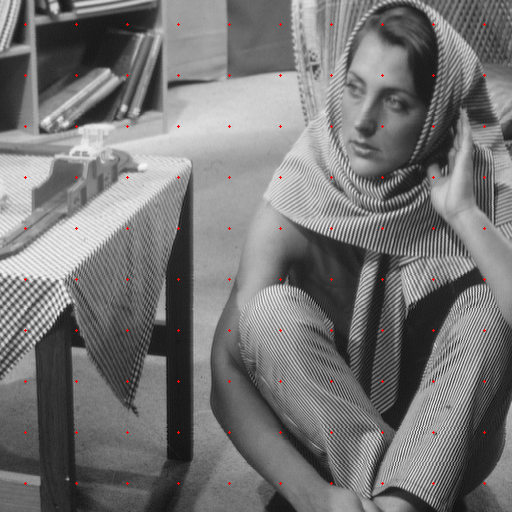
\includegraphics[width=0.6\textwidth]{img/spatiallyUniformSampling.png}
      \caption{Spatially uniform sampling. Red pixels are sampled. Here 100 pixels are sampled, which only represents 0.04\% of all pixels.}
  \end{figure}
 \item [Incremental sampling (INS)] is an adaptive sampling scheme, meaning that it select points according to the similarity, so that we can have an approximate optimal rank-k subspace of the original image \cite{zhan_improved_2017}.
 \item [Mean-shift segmentation-based sampling] this scheme performs good for complex backgrounds. The method consists in over-segmenting the image into \(n\) regions and only one pixel of each region will be sampled using the spatially closest pixel to the center of the region given a formula in \cite{kao_sampling_2012}.
\end{description}

\subsection{Affinity function}

\paragraph{}
The kernel function measures the similarity between the pixel \(y_i\) and \(y_j\).
The chosen function is important because it decides on which features the similarity of pixels will be evaluated.
Some of the most used affinity functions are:

\begin{description}[align=left]
 \item [Spatial Gaussian Kernel] takes only into account the spatial distance between two pixels \cite{siam_slides_2016}.
  The formula of this kernel is, with \(\forall i, j \in [1, N]\), \(x_i\) the coordinate vector of a pixel and \(h_x\) a normalisation parameter,
  \[K(y_i, y_j) = exp(-\frac{||x_i - x_j||^2}{h_x^2}).\]
  The parameter is influencing on the normalisation of the values and gaussian standard deviation.
  The greater it is, the more tolerant the spatial distance computation will be.

 \item [Photometric Gaussian Kernel] considers the intensity and color similarity of the pixels \cite{siam_slides_2016}.
  The formula of this kernel is, with \(z_i\) the color or grayscale of a pixel,
  \[K(y_i, y_j) = exp(-\frac{||z_i - z_j||^2}{h_z^2}).\]
  Generally, the \(h\) parameter is a smoothing parameter.
  If \(h\) is small, it is more discriminating between the affinity of different pixels.

 \item [Bilateral Kernel] one of the most used kernel which smooths images by a nonlinear combination of the spatial and photometric gaussian kernels \cite{siam_slides_2016} \cite{glide_2014} \cite{bilateral_tomasi_1998}:
  \[K(y_i, y_j) = exp(-\frac{||x_i - x_j||^2}{h_x^2}) exp(-\frac{||z_i - z_j||^2}{h_z^2}).\]

  To generate the example below, we use the famous grayscale image of Barbara of size \(512 \times 512\) pixels.
  The more a pixel is colored in red, the more similar it is to the selected pixel, with respect to the chosen bilateral kernel.
  A blue colored pixel is dissimilar to the considered pixel.
  We use a spatially uniform sampling technique and select 0.1\% of the pixels.
  These are two affinity vectors, the first one is of a pixel on the table leg and the second around Barbara's eye.
  Keep in mind that each affinity image shown represents only one row of the affinity matrix\ \(K\).

  \begin{figure}[H]
      \centering
      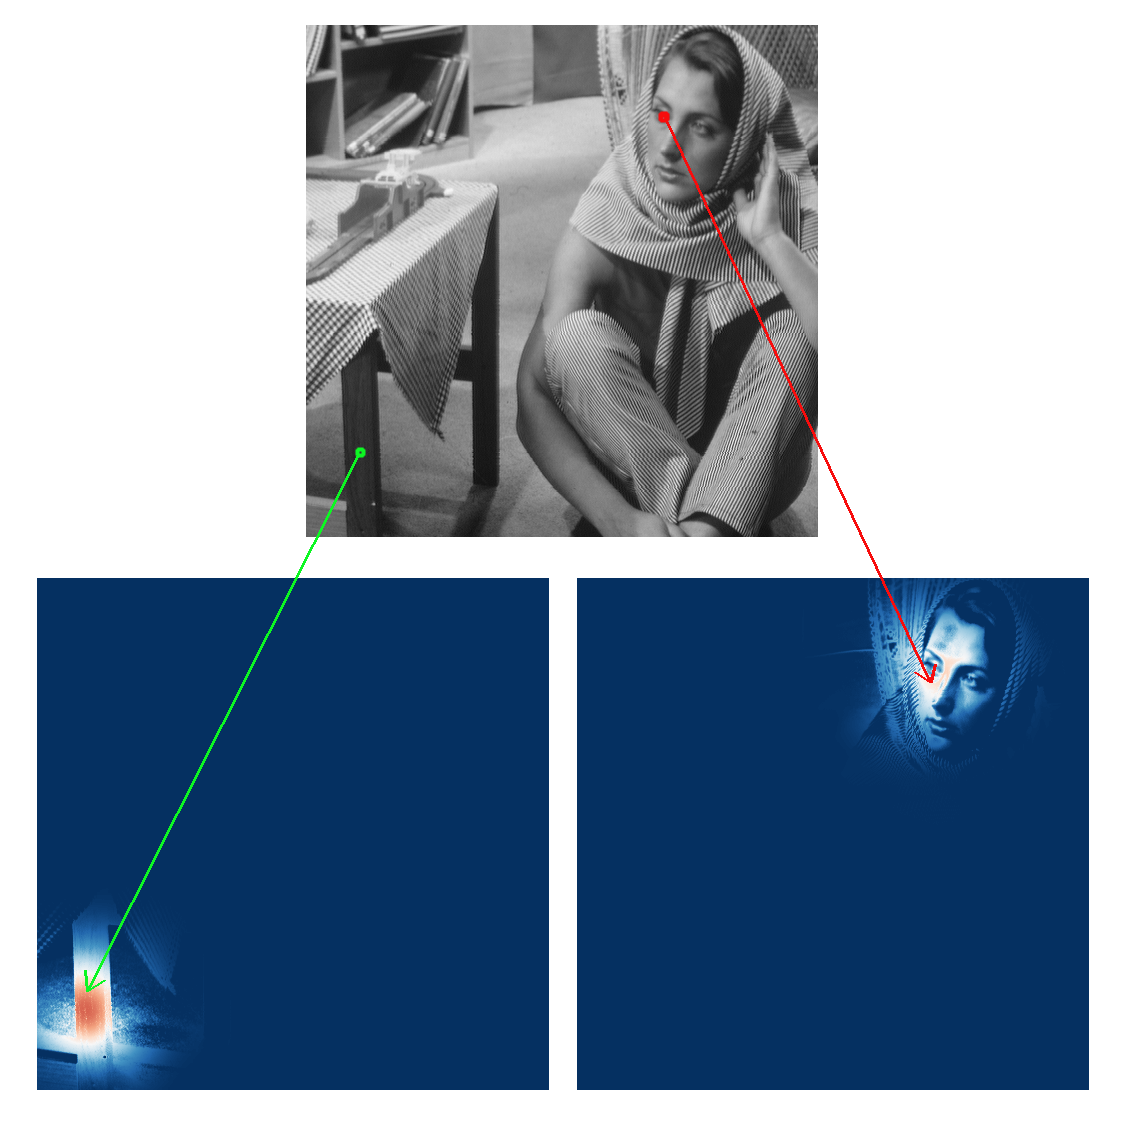
\includegraphics[width=\textwidth]{img/bilateralAffinityPhoto35Spatial50.png}
      \caption{Affinity matrices with \(h_x = 50\) and \(h_z = 35\).}
  \end{figure}
  In a very heterogeneous image, the bilateral kernel will be useful to keep the spatial similarity, but with excluding very dissimilar neighbour pixels.

 \item [Non-Local Means (NLM)] is similar to the bilateral kernel, a data-dependent filter, except that the photometric affinity is captured patch-wise \cite{glide_2014} \cite{kervrann_nlm_2006}.
 \item [Locally Adaptive Regression Kernel (LARK)] uses the geodesic distance based on estimated gradients \cite{milanfar_symmetrizing_2013} \cite{takeda_kernel_2007}.
\end{description}

\subsection{Graph Laplacian operator}

\paragraph{}
The graph Laplacian operator has multiple possible definitions and each has its own properties.
A good summary can be found in \cite{siam_slides_2016}.
A graph Laplacian can be symmetric which is important for the eigendecomposition of the matrix.
The spectral range, corresponding to the range of the eigenvalues, is important because we can use the filters derived from the Laplacian multiple times, and if the eigenvalues are not between 0 and 1, then the filters tend to be unstable.
With \(K\) being the affinity matrix, \(d_i = \sum_j K_{ij}\) and \(D = diag\{d_i\}\):

\begin{table}[!htbp]
 \centering
 \begin{tabular}{|c|c|c|c|c|}
  \hline
  Laplacian Name & Formula & Symmetric & Spectral Range \\
  \hline
  Un-normalised & \(D - K\) & Yes & [0, n] \\
  \hline
  Normalised & \(I - D^{-1/2}KD^{-1/2}\) & Yes & [0, 2] \\
  \hline
  Random Walk & \(I - D^{-1}K\) & No & [0, 1] \\
  \hline
  ``Sinkhorn" \cite{milanfar_symmetrizing_2013} & \(I - C^{-1/2}KC^{-1/2}\) & Yes & [0, 1] \\
  \hline
  Re-normalised \cite{milanfar_new_2016} & \(\alpha(D - K)\), \(\alpha = \bigO(N^{-1})\) & Yes & [0, n] \\
  \hline
 \end{tabular}
\end{table}
Generally, it is a good practice to stick to one definition of the Laplacian.

\section{Implementation}

\subsection{Algorithm specifications}
In our algorithm, we shall use spatially uniform sampling for the ease of implementation and robustness.
The kernel function is the bilateral one.

\subsection{Implementation}

\paragraph{Prototyping}
Python

\paragraph{Parallel implementation}
PETSc

\paragraph{Inverse subspace iteration}
%\cite{stuff}

\subsection{Results}
TODO some results (image processing) + performances (for GMRES + ASM)
